\documentclass[hyperref=unicode,utf8,xcolor=pst]{beamer}
\usetheme{boxes}
\setbeamertemplate{navigation symbols}{}
%
\definecolor{mirantisred}{RGB}{211,48,26}
\setbeamercolor{titlelike}{fg=mirantisred}
\setbeamercolor{structure}{fg=mirantisred}
%
\usepackage[T2A]{fontenc}
%
\usepackage{graphicx}
\usepackage{fancyvrb}
%
% Copyright (c) 2014  Mirantis, Inc.
%
%    Licensed under the Apache License, Version 2.0 (the "License"); you may
%    not use this file except in compliance with the License. You may obtain
%    a copy of the License at
%
%         http://www.apache.org/licenses/LICENSE-2.0
%
%    Unless required by applicable law or agreed to in writing, software
%    distributed under the License is distributed on an "AS IS" BASIS, WITHOUT
%    WARRANTIES OR CONDITIONS OF ANY KIND, either express or implied. See the
%    License for the specific language governing permissions and limitations
%    under the License.
%
\title{Ceph in Mirantis OpenStack}
%\author{
\includegraphics[height=4cm, trim=3cm 2cm -5cm 4cm, clip]{Vector_RGB_MirantisLogo}\\Dmitry Borodaenko}
\author{
\includegraphics[height=5cm]{Vector_RGB_MirantisLogo}\\Dmitry Borodaenko}
\date{Mountain View, 2014}
%
\begin{document}

\begin{frame}
	\titlepage
\end{frame}

\begin{frame}
	\setcounter{framenumber}{1}
	\frametitle{\insertframenumber{}. The Plan}
	\begin{enumerate}
		\item What is Ceph?
		\item How does Ceph fit into OpenStack?
		\item What can you make Ceph do with Fuel?
		\item Gotchas and limitations
		\item Ceph architecture overview
		\item Storage architecture for OpenStack with Ceph
		\item Deploying Ceph with Mirantis OpenStack
		\item Operating Ceph backed OpenStack services
		\item Troubleshooting
		\item Resources
	\end{enumerate}
\end{frame}

\begin{frame}
	\frametitle{\insertframenumber{}. What is Ceph?}
	Ceph is a free storage system that provides unified object,
	block, and file storage.

	\begin{description}
		\item[Object Storage] RADOS objects support
			snapshotting, replication, and consistency.
		\item[Block Storage] RBD block devices are thinly
			provisioned over RADOS objects and can be
			accessed by QEMU via librbd library.\\
			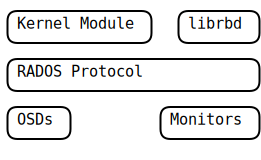
\includegraphics[height=2.5cm]{ceph-rbd}
		\item[File Storage] CephFS metadata servers (MDS)
			provide a POSIX-compliant overlay over RADOS.
	\end{description}
\end{frame}

\begin{frame}
	\frametitle{\insertframenumber{}. What is Mirantis OpenStack?}

	\begin{description}
		\item[OpenStack] is an open source cloud computing
			platform.\\
			\vspace{0.5ex}
			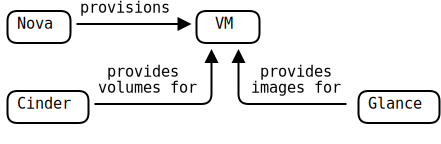
\includegraphics[height=1.9cm]{openstack-components}
		\item[Mirantis] ships hardened OpenStack packages and
			provides Fuel utility to simplify deployment of
			OpenStack.
		\item[Fuel] uses Cobbler, MCollective, and Puppet to
			discover nodes, provision OS, and setup
			OpenStack services.\\
			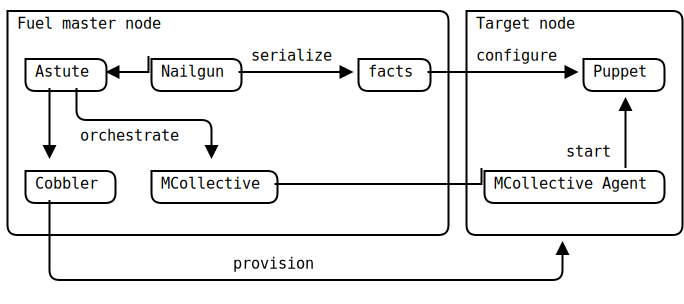
\includegraphics[height=3.7cm]{fuel-components}
	\end{description}
\end{frame}

\begin{frame}
	\frametitle{\insertframenumber{}. How does Ceph fit into
	OpenStack?}
	\begin{columns}
		\column{.65\textwidth}
		RBD drivers for OpenStack make libvirt configure the
		QEMU interface to librbd.

		\vspace{2ex}
		Ceph benefits:
		\begin{itemize}
			\item Multi-node striping and redundancy for
				block storage (Cinder volumes and Nova
				ephemeral drives)
			\item Copy-on-write cloning of images to
				volumes and instances
			\item Unified storage pool for all types of
				storage (object, block, POSIX)
			\item Live migration of Ceph-backed instances
		\end{itemize}

		\column{.35\textwidth}
		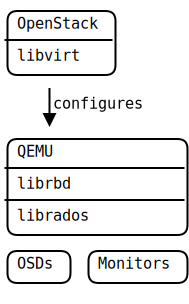
\includegraphics[height=6.5cm]{ceph-rbd-openstack}
	\end{columns}
\end{frame}

\begin{frame}
	\frametitle{\insertframenumber{}. What has Fuel ever done for Ceph?}

	\begin{enumerate}
		\item Deploys Ceph Monitors and OSDs on dedicated nodes
			or in combination with OpenStack components.\\
			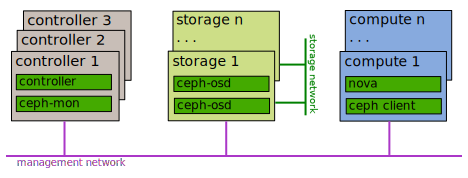
\includegraphics[height=3.7cm]{openstack-nodes}
		\item Creates partitions for OSDs when nodes are
			provisioned.
		\item Creates separate RADOS pools and sets up Cephx
			authentication for Cinder, Glance, and Nova.
		\item Deploys RADOS Gateway (S3 and Swift API frontend
			to Ceph) behind HAProxy on controller nodes.
	\end{enumerate}
\end{frame}

\end{document}
